\documentclass[3p,review]{elsarticle}

\usepackage{lineno,hyperref}
%\usepackage{amsmath}
%\usepackage{arydshln}
\usepackage{subcaption}
%\usepackage{subfigure}
\usepackage{comment,color}


\usepackage{graphicx,amsfonts,url,multirow}
%\usepackage[cmex10]{amsmath}
\modulolinenumbers[5]

\journal{Information Fusion}

\newcommand{\TODO}{\textbf{TODO}}

%%%%%%%%%%%%%%%%%%%%%%%%%%%%%%%%%%%%%%%%%%%%%%%%%%%%%%%%%%%%%%%%%%%%%%%%%%%%%%%%%%%%%%%%%

\begin{document}

\begin{frontmatter}

\title{Big Data Analytics: A Tutorial on Information Process Fusion with MapReduce}

\author[grx]{Sergio Ram\'irez\corref{cor1}}
\ead{sramirez@decsai.ugr.es}

\author[grx]{Alberto Fern\'andez}
\ead{alberto@decsai.ugr.es}

\author[grx]{Salvador Garc\'ia}
\ead{salvagl@decsai.ugr.es}

\author[grx]{Francisco Herrera}
\ead{herrera@decsai.ugr.es}

\address[grx]{Department of Computer Science and Artificial Intelligence, University of Granada, Granada, Spain}
%\address[kau]{Faculty of Computing and Information Technology - North Jeddah, King Abdulaziz University (KAU), Jeddah, Saudi Arabia}


\cortext[cor1]{Corresponding author. Tel:+34-958-240598; Fax: +34-958-243317}

\begin{abstract}

\TODO

%In this paper we aim at presenting the first outcomes in this framework, and to analyze the behavior of standard solutions to address imbalanced classification in Big Data problems. The features of these recent approaches, and the experimental results obtained throughout this work, will allow us to determine the current state of this area of research and to provide a discussion on the future directions. 

\end{abstract}

\begin{keyword}
Big Data Analytics, MapReduce, Information Fusion, Spark, Machine Learning
\end{keyword}

\end{frontmatter}

\section{Introduction}\label{sec:intro}

\TODO

In order to address all these objectives, this paper is organized as follows. First, Section \ref{sec:mr} presents an introduction on the MapReduce programming framework, also stressing some alternatives for Big Data processing. Section \ref{sec:techno} includes an overview on those technologies currently available to address Big Data problems from a distributed perspective. Section \ref{sec:fusion} presents the core of this paper, analyzing the different design options for developing Big Data analytics algorithms regarding how the partial data and models are aggregated. Then, we show a case study in Section \ref{sec:exp} to contrast the capabilities regarding scalability of the different approaches previously introduced. Finally, Section \ref{sec:conclusions} summarizes and concludes this paper.

\section{MapReduce as Information Process Fusion}\label{sec:mr}




INTRO

\subsection{MR}\label{subsec:mr}

The rapid growth and influx of data from private and public sectors has popularized the notion of ``Big data \cite{Fer14}''. The surge in Big Data has led to the development of custom models and algorithms that are able to extract significant value and insight in different areas such as medical, health care, business, management and so on \cite{Kam14,Chen14,Wu14}.

In order to to provide robust and scalable solutions, new research paradigms and developmental tools have been made available. These frameworks have been designed to ease both the storage necessities and the processing of Big Data problems \cite{Fer14}. 

The MapReduce execution environment \cite{Dea08} is the most common framework used in this scenario. Being a privative tool, its open source counterpart, known as Hadoop, has been traditionally used in academia research \cite{Whi15-Hadoop}. It has been designed to allow distributed computations in a transparent way for the programmer, also providing a fault-tolerant execution scheme. To take advantage of this scheme, any algorithm must be divided into two main stages: Map and Reduce. The first one is devoted to split the data for processing, whereas the second collects and aggregates the results.

Additionally, the MapReduce model is defined with respect to an essential data structure: the $<$key,value$>$ pair. The processed data, the intermediate and final results work in terms of $<$key,value$>$ pairs. To summarize its procedure, Figure \ref{fig:mapreduce} illustrates a typical MapReduce program with its \textit{Map} and \textit{Reduce} steps. The terms $k_i:v_j$ refer to the key and value pair that are computed within each Map process. Then, values are grouped linking them to the same key, i.e. $k_i:v_j,\ldots, v_h$, and feed to the same Reduce process. Finally, values are aggregated with any function within the Reduce process to obtain the final result of the algorithm.

%\begin{comment}
\begin{figure}[!ht]
\centering \resizebox{0.75\textwidth}{!}{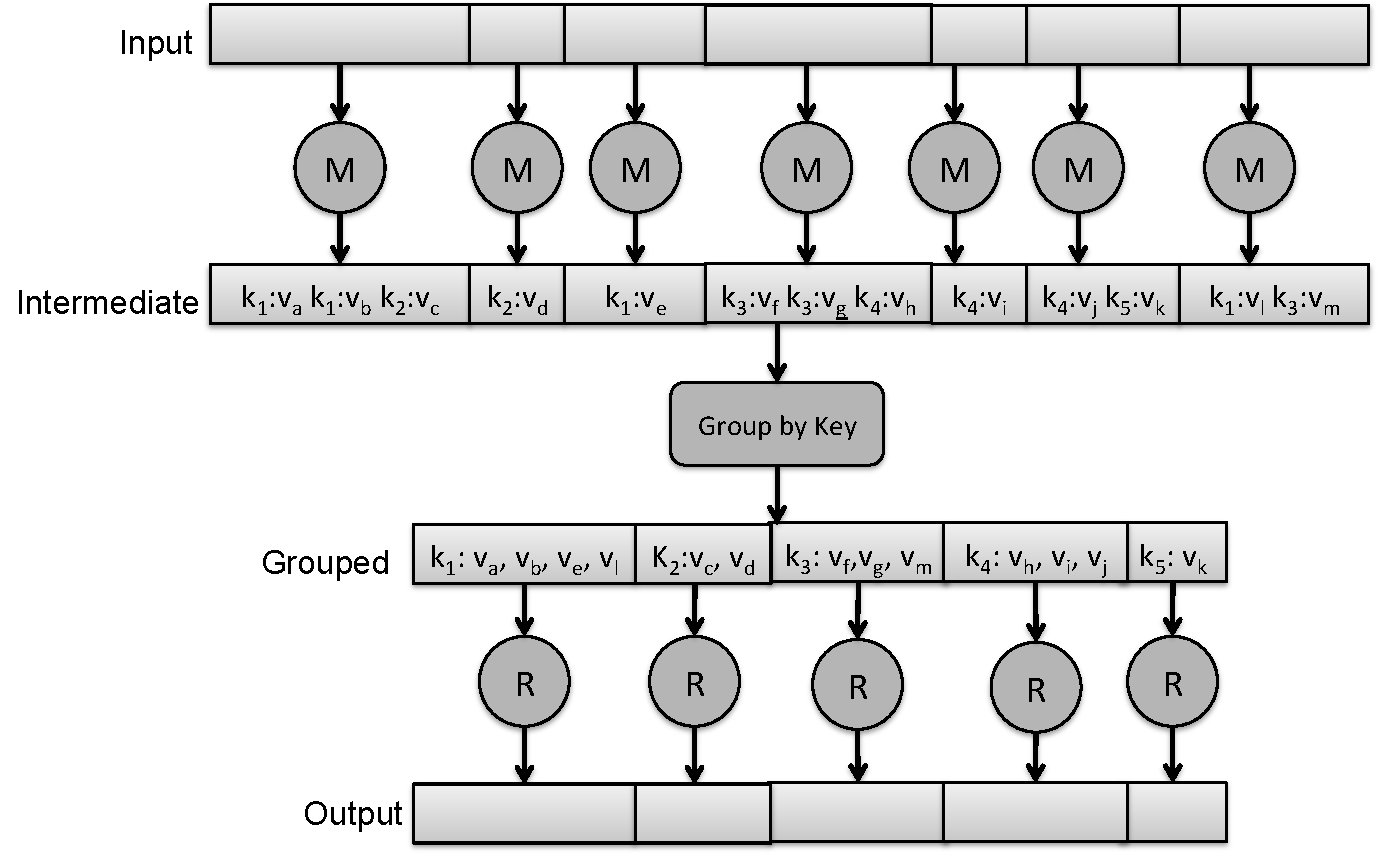
\includegraphics{mapreduce}} \caption{The MapReduce programming model.}
\label{fig:mapreduce}
\end{figure}
%\end{comment}

From this initial model, more recent alternative frameworks have arisen to provide more efficient computations for iterative process, which are the basis for any Machine Learning algorithm. Among them, Apache Spark \cite{Zaharia12,Zaharia10} is clearly emerging as a more commonly embraced platform for implementing Machine Learning solutions that scale with Big Data.

\subsection{Alternatives}\label{subsec:altMR}

\TODO

\section{Big Data Technologies for Analytics}\label{sec:techno}

\TODO

\subsection{Hadoop}\label{subsec:hadoop}

\TODO

\subsection{Spark}\label{subsec:spark}

Apache Spark Framework~\cite{spark} was born in 2010 with the publication of Resilient Distributed Datasets (RDD) structures~\cite{zaharia12}, the key idea behind Spark. Although ASF has a close relationship with many components from Hadoop Ecosystem, Spark provides specific support for every step in the Big Data stack, such as its own processing engine, and machine learning library. 

Apache Spark~\cite{hamstra15} can be defined as a distributed computing platform which can process large volume data sets in memory with a very fast response time, thanks to its memory-intensive scheme. It was originally thought to tackle problems deemed as unsuitable for previous disk-based engines like Hadoop. Continued use of disk is replaced in Spark by memory-based operators that efficiently deal with iterative and interactive problems (prone to multiple I/O actions). 

%RDD
The heart of Spark is formed by Resilient Distributed Datasets (RDD), which transparently controls how data are distributed and transformed across the cluster. Users just need to define some high-level functions that will be applied and managed by RDDs. These elements are created whenever data are read from any source, or as a result of a transformation. RDDs consist of a collection of data partitions distributed across several data nodes. A wide range of operations are provided for transforming RDDs, such as: filtering, grouping, set operations, among others. Furthermore RDDs are also highly versatile as they allows users to customize partitioning for an optimized data placement, or to preserve data in several formats and contexts.

% lineage
In Spark, fault tolerance is solved by annotating operations in a structure called lineage. Spark transformations annotated in the lineage are only performed whenever a trigger I/O operations appears in the log. In case of failure, Spark re-computes the affected brach in the lineage log. Although replication is normally skipped, Spark allows to spill data in local disk in case the memory capacity is not sufficient. 

%Dataframes
Spark developers provided another high-level abstraction, called DataFrames, which introduces the concept of formal schema in RDDs. DataFrames are distributed and structured collections of data organized by named columns. They can be seen as a table in a relational database or a dataframe in R, or Python (Pandas). As a plus, relational query plans built by DataFrames are optimized by the Spark's Catalyst optimizer throughout the previously defined schema. Also thanks to the scheme, Spark is able to understand data and remove costly Java serialization actions.

%Datasets
A compromise between structure awareness and the optimization benefits of Catalyst is achieved by the novel Dataset API. Datasets are strongly typed collections of objects connected to a relational schema. Among the benefits of Datasets, we can find compile-time type safety, which means applications can be sanitized before running. Furthermore, Datasets provide encoders for free to directly convert JVM objects to the binary tabular Tungsten format. These efficient in-memory format improves memory usage, and allows to directly apply operations on serialized data. Datasets are intended to be the single interface in future Spark for handling data.

\subsubsection{MLlib}


MLlib project~\cite{mllib15} was born in 2012 as an extra component of Spark. It was released and open-sourced in 2013 under the Apache 2.0 license. From its inception, the number of contributions and people involved in the project have been growing steadily. Apart from official API, Spark provides a community package index~\cite{sparkpackages} (Spark Packages) to assemble all open source algorithms that work with MLlib. 

MLlib is a Spark library geared towards offering distributed machine learning support to Spark engine. This library includes several out-of-the-box algorithms for alike tasks, such as: classification, clustering, regression, recommendation, even data preprocessing. Apart from distributed implementations of standard algorithms, MLlib offers:

\begin{itemize}
	\item Common Utilities: for distributed linear algebra, statistical analysis, internal format for model export, data generators, etc. 
	\item Algorithmic optimizations: from the long list of optimizations included, we can highlight some: decisions trees, which borrow some ideas from PLANET project~\cite{panda09} (parallelized learning both within trees and across them); or generalized linear models, which benefit from employing fast C++-based linear algebra for internal computations.
	\item Pipeline API: as the learning process in large-scale datasets is tedious and expensive, MLlib includes an internal package (\emph{spark.ml}) that provides an uniform high-level API to create complex multi-stage pipelines that connect several and alike components (preprocessing, learning, evaluation, etc.). \emph{spark.ml} allows model selection or hyper-parameter tuning, and different validations strategies like k-fold cross validation.
	\item Spark integration: MLlib is perfectly integrated with other Spark components. Spark GraphX has several graph-based implementations in MLlib, like LDA. Likewise, several algorithms for online learning are available in Spark Streaming, such as online k-Means. In any case, most of component in the ASF stack are prepared to effortlessly cooperate with MLlib.
\end{itemize}

\subsection{Flink}\label{subsec:flink}

Apache Flink~\cite{flink} is a distributed processing component focused on streaming processing, which was designed to solve problems derived from micro-batch models (Spark Streaming). Flink also supports batch data processing with programming abstractions in Java and Scala, though it is treated as a special case of streaming processing. In Flink, every job is implemented as a stream computation, and every task is executed as cyclic data flow with several iterations. 

Flink provides two operators for iterations~\cite{flinkengine}, namely, standard and delta iterator. In standard iterator, Flink only works with a single partial solution, whereas delta iterator utilizes two worksets: the next entry set to process and the solution set.
Among the set of advantages provided these iterators is the reduction of data to be computed and sent between nodes \cite{EwenTKM12}. According to the authors, new iterators are specially designed to tackle machine learning and data mining problems.

Apart from iterators, Flink leverages from a PACT optimizer which analyzes the code and the data access conflicts to reorder operators and create semantically equivalent execution plans~\cite{Alexandrov14,Hues12}. Physical optimization is then applied on plans to boost data transport and operators' execution on nodes. Finally, PACT optimizer selects the most resource-efficient plan, regarding network and storage.

Furthermore, Flink provides a complex fault tolerance mechanism to consistently recover the state of data streaming applications. This mechanism is generating consistent snapshots of the distributed data stream and operator state. In case of failure, the system can fall back to these snapshots.

FlinkML is aimed at providing a set of scalable ML algorithms and an intuitive API to Flink users. Until now, FlinkML provides few alternatives for some fields in machine learning: SVM with CoCoA or Multiple Linear regression for supervised learning, k-NN join for unsupervised learning, scalers and polynomial features for preprocessing, Alternating Least Squares for recommendation, and other utilities for validation and outlier selection, among others. FlinkML also allows users to build complex analysis pipelines via chaining operations (like in MLlib). FlinkML pipelines are inspired by the design introduced by sklearn in~\cite{buitin13}.

\section{Big Data Analytics on Fusion Process}\label{sec:fusion}

\TODO

\subsection{Direct fusion of models: ensemble approach}\label{subsec:ensemble}

\TODO

\subsection{Approximate fusion of models: aggregation of partial systems}\label{subsec:submodels}

\TODO

\subsection{Exact fusion for scalable models: distributed data and models' partition}\label{subsec:exact}

\TODO

\section{Practical Study on XXX}\label{sec:exp}

\TODO



\section{Concluding Remarks}\label{sec:conclusions}

\TODO

\section*{Acknowledgments}\label{sec:ack}

This work have been partially supported by the Spanish Ministry of Science and Technology under projects TIN2014-57251-P and TIN2015-68454-R; and the Foundation BBVA project 75/2016 BigDaPTOOLS.
%\newline

%\noindent\appendix{\textbf{Bibliography}}\label{sec:biblio}

\bibliographystyle{elsarticle-num}
\bibliography{cloud,sergio}

\end{document}
